\section{Overview}
\label{sec:goals}

We would like to develop software security solutions that are widely
applicable and offer strong guarantees. We take a binary-centric
approach to software security because binary code is everywhere, and
binary code is faithful to what will actually be executed on
hardware. Effective security-centric binary analysis techniques thus
can potentially impact a wide audience, and provide strong guarantees
as to what will actually be executed.


There are potentially many types of security analysis we want to
perform on binary programs.  Several scenarios in which we have used
binary program analysis include:
\begin{itemize}\squish
\item {\bf Input Filter Generation.}  In input filter generation, we
  use program analysis to generate a recognizer for the set of inputs
  that trigger a vulnerability (Chapter~\ref{chap:filters}). These
  recognizers are called filters (also sometimes called signatures)
  because of how they are used. If the recognizer matches an input,
  the input is considered an exploit and is filtered (dropped).
  Filters allow even vulnerable programs to continue to operate as
  normal under attack because all exploits are filtered. 

\item {\bf Automatic Patch-Based Exploit Generation.}  In automatic
  patch-based exploit generation (APEG) (Chapter~\ref{chap:apeg}), we
  are given a vulnerable program $P$ and a patched version $P'$. The
  goal is to generate an input that triggers the vulnerability in $P$
  that was patched in $P'$.  If APEG is possible, this would imply
  that patches may not always help security since attackers can use
  them to generate exploits.  

\item {\bf Automatic Deviation Detection.}  In automatic deviation
  detection (Chapter~\ref{chap:others}), we are given two
  implementations $A$ and $B$ of the same specification. The goal is
  to generate an input that will cause the behavior of $A$ to deviate
  from $B$. We can use such inputs to differentiate the two
  implementations, i.e., the inputs act as a ``fingerprint'' which
  distinguish the two implementations.

\item {\bf Reverse Engineering.}  Reverse engineering is the process
  of recovering higher level semantics from low-level code.  For
  example, we may want to reverse engineer a proprietary network
  protocol (Chapter~\ref{chap:reverse}), determine whether a program
  has malicious behavior (Chapter~\ref{chap:malware}), and uncover
  trigger-based behavior (Chapter~\ref{chap:trigger}). Reverse
  engineering allows us to extract important information from a
  program binary. 

\item {\bf Determine the Ground Truth.}  A binary code is the ground
  truth of the instructions issued to the hardware.  One may think
  that since binary code is compiled from a higher-level language that
  analysis on the higher-level language will transitively carry over
  to the binary code. Unfortunately, this is not true.  One problem is
  a language may support abstractions that are not enforced during
  execution, e.g., protection such as {\tt private} and {\tt
    protected} for class members is not enforced at the binary level
  --- anyone can call these members if they know the instruction
  address. Another problem is the compiler may remove
  security-critical code. One well known example is highlighted in the
  following code:
  \begin{small}
  \begin{code}
1. get\_password(password);
2. do\_secret\_stuff(password);
3. memset(password, 0, sizeof(password)); 
4. ...
  \end{code}
  \end{small}
  The final {\tt memset} is intended to zero-out the user-supplied {\tt
    password} in order to minimize the amount of time a user password
  is in memory.  For example, the author may assume that any program
  crash after line 3 will not contain the user password as part of the
  crash dump file. However, certain compilers will remove the call to
  {\tt memset} as part of program optimization~\cite{howard:2002}.
\end{itemize}


Although the end security goal is different in each problem instance,
all are possible by analyzing the binary program.  Furthermore, the
problem instances share many similarities. For example, in each
scenario above we 1) need to parse a binary file into a sequence of
executed instructions, 2) accurately model the potential effects of
each instruction that maybe executed, and 3) analyze how control and
data flow between instructions.  The commonality between problems
motivates the design of a single binary analysis platform.
However, in order to take a binary-centric approach, we need tools and
techniques that are capable of analyzing binary code.

\paragraph{Binary Analysis is Challenging.} One challenge to binary
analysis is dealing with the engineering issues that arise from
real-world code.  A typical program analysis consists of first writing
logic for each type of program instruction, then iterating the logic
over all program instructions. Modern architectures such as x86 have
hundreds of different instructions, each of which has complicated
semantics.  We would like to engineer a solution that does not require
a programmer to consider each of the hundred complex cases
individually for each desired program analysis.


A second challenge is that binary program analysis is different than
program analysis for typical higher-level languages. While
higher-level languages have types, functions, pointers, loops, and
local variables, assembly has \emph{no types, no functions, one
  globally addressed memory region, goto's and stack frames instead of
  local variables}.  


One may think that we simply need to infer the higher-level
information from the binary, i.e., decompile the binary code to the
source code. However, there are several problems with this
approach. First, it assumes that compilation is an invertible
function.  Compilation tends to be a many-to-one process, e.g., many
variables are compiled down to a few registers, many pointers become
one global memory, many user-defined types are compiled down to the
integer register types, etc. The many-to-one relationship means
fundamentally some information is lost during compilation.  Second,
source-code tends to have abstractions not present in binary code,
thus there is no reason to believe we can re-infer them.  Third, the
compilation process may want to explicitly violate abstractions for
efficiency. For example, tail-recursion
optimizations~\cite{muchnick:1997} may result in violating the stack
discipline because a call does not return to the callee. Finally,
decompilation tends to require we know the original source code
language, thus excludes analyzing hand-generated assembly.




\subsection{Overview of the \bap Binary Analysis Platform}

The \bap platform is designed to facilitate faithful
security-relevant binary program analysis.  At the core of \bap is an
intermediate language (IL) which treats assembly as a first-class
language. The IL abstracts away platform-specific details in order to
make writing analysis easy, while enabling fine-grained reasoning
about the instructions the processor may execute.  Thus, \bap is
appropriate where other tools and techniques may fail or be too
imprecise.  For example, we build a decompiler on top of \bap, but a
decompiler itself may be unsuitable for analyzing malware where
higher-level program abstractions are broken on purpose in an effort
to fool analysis.

\begin{figure}
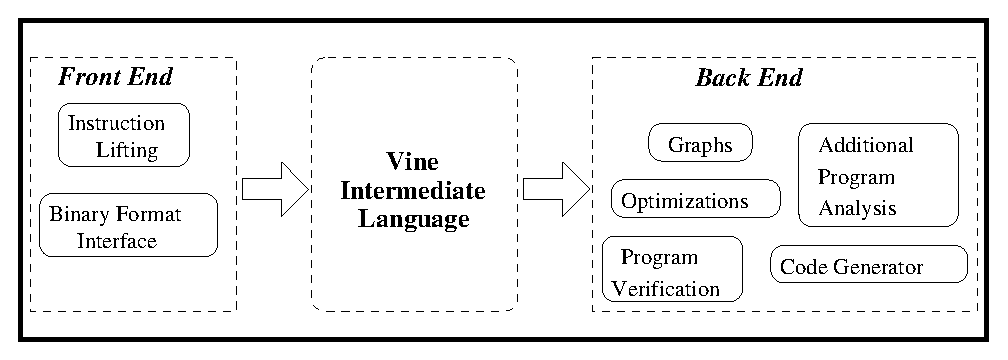
\includegraphics{fig/vine-components}
\caption{The\bap binary analysis architecture and components. \bap
  is divided into a front-end, which is responsible for lifting
  instructions to the \bap intermediate language, and a back end
  responsible for analysis.}
\label{fig:vine-components}
\end{figure}

A high-level picture of the \bap binary analysis platform is shown in
Figure~\ref{fig:vine-components}.  \bap is roughly divided up into a
front-end and back end.  At a high level, the front end is
architecture-specific, and responsible for accessing the raw bits in
the binary file and lifting disassembled instructions to the \bap
IL. The back-end is architecture-independent, and is where all
analysis is performed.

\bap is designed around several principles:
\begin{itemize}\squish

\item {\bf Ease of Writing Analysis.}  A typical program analysis
  consists of first writing logic that reasons about each particular
  kind of instruction that may be executed, e.g., binary operations,
  unary operations, stores, loads, etc., and then iterating the logic
  over each possible instruction. We simplify the process of writing
  such analysis by providing a single, simplified IL, as well as
  common routines such as iterating over all instructions.

\item {\bf Correctness.}  Once a program analysis is written, we would
  like to make it easy to verify that it is correct. Typically we
  verify that a program is correct by arguing either soundness or
  completeness of the analysis.  A soundness argument states that
  whatever the program analysis says is true must really be true, and
  a completeness argument states that whatever is true the program
  analysis will say.  \bap facilitates correctness arguments by
  having a formally defined semantics.

\item {\bf Distinguish What is Known from What Is Not.}  In practice,
  our implementation may not always be complete.  For example, \bap
  may not handle some instructions for an architecture because doing
  so would require significant implementation.  Instead of silently
  ignoring such cases, \bap explicitly differentiate between what is
  handled by the infrastructure and what is not.

\item {\bf Platform Agnostic.} Binary code is everywhere, but there is
  more than one architecture. In order for our techniques and
  implication to be as widely applicable as possible, we would like to
  support as many architectures as possible.  We have designed \bap
  similar to a compiler in order to address this goal.  \bap has a
  front-end which is architecture-specific, and an
  architecture-independent back-end. As a result, analysis themselves
  are universal to any architecture that is lifted to the \bap IL.
  If we wish to support a new architecture, we only need to port the
  front end.

\item {\bf Modularity.}  Our main goal is to solve security
  goals. Thus, we would like to use existing research and components
  when appropriate.  \bap is designed to in a modular fashion in
  order to take advantage of existing tools and techniques where
  possible. For example, \bap itself does not disassemble: we use
  existing disassemblers to parse instructions. \bap is responsible
  for lifting the instruction up to the IL, and all analysis on the
  IL.  For instance, we have used \bap to construct a certifying
  disassembler that can certify disassembled code paths are executable
  (Chapter~\ref{chap:provable-disassemble}).

\end{itemize}





